\chapter{Call Signatures for Persistence Techniques}\label{chapter:call signatures for persistence techniques}
In this chapter, we will write Call Signatures (introduced in \autoref{chapter:call signatures}) to describe function calls used in four of the commonly implemented persistence techniques (from \autoref{chapter:persistence techniques}). In \autoref{chapter:experiments}, we will use these Call Signatures to detect persistence techniques in real-world malware samples and to analyze the effectiveness of Call Signatures.

\medskip

We introduced four categories of persistence techniques in \autoref{chapter:persistence techniques} (directory-based, Registry-based, service-based, and scheduled task-based techniques). We first analyze what function calls are made to implement these persistence techniques, and we then look at how we can express these function calls as Call Signatures.

\begin{itemize}
    \item In \autoref{section:call signatures rp}, we write Call Signatures for \autoref{RP0}.
    \item In \autoref{section:call signatures dp}, we write Call Signatures for \autoref{DP0}.
    \item In \autoref{section:call signatures sp}, we write Call Signatures for \autoref{SP0}.
    \item In \autoref{section:call signatures tp}, we write Call Signatures for \autoref{TP0}.
\end{itemize}

Finally, in \autoref{section:reflection on writing call signatures}, we reflect on writing Call Signatures.

\section{Registry-based Persistence Techniques}\label{section:call signatures rp}
In this section, we will discuss Call Signatures for \autoref{RP0}, a technique that writes to (a subkey of) the Registry key \path{HKCU\SOFTWARE\Microsoft\Windows\CurrentVersion\Run}.

As we saw in \autoref{section:background windows registry}, there are two common ways for applications to modify the Registry, namely the Windows API and the \texttt{reg.exe} command-line application.

\subsection{Modifying the Registry via the API}

To set the value in a Registry key using the Windows API, an application first needs to (create or) open it using one of the following functions (as seen in the examples in \autoref{appendix:source code run time linking}):
\begin{multicols}{2}
  \begin{itemize}
      \item \texttt{RegCreateKey}
      \item \texttt{RegCreateKeyEx}
      \item \texttt{RegOpenKey}
      \item \texttt{RegOpenKeyEx}
  \end{itemize}
\end{multicols}

All of these functions work similarly. The first argument takes a constant that specifies the root key. For example, the constant \texttt{0x80000001} represents \texttt{HKCU}. The second argument specifies the path of the key.

To detect \autoref{RP0} we need to find a call to a function where the first parameter is \texttt{0x80000001} and the second argument contains ``\path{SOFTWARE\Microsoft\Windows\CurrentVersion\Run}''. \autoref{listing:call signature run key windows api} is a Call Signature for such calls.

\begin{lstlisting}[label={listing:call signature run key windows api}, caption={A Call Signature for \autoref{RP0}.}, captionpos=b]
---

signature:
  technique: "RP0"
  description: >
      This Call Signature can be used to
      search for calls to RegCreateKey or RegOpenKey,
      that are used to implement RP0.
  rules:
      - element: "function name"
        contains_in:
          - "RegCreateKey"
          - "RegOpenKey"

      - element: "number of arguments"
        equals: 3

      - element: "argument"
        argument_index: 0
        equals: 0x80000001

      - element: "argument"
        argument_index: 1
        contains: "SOFTWARE\\Microsoft\\Windows\\CurrentVersion\\Run"
\end{lstlisting}

\subsection{Modifying the Registry via Reg.exe}
To modify the Windows Registry using \texttt{reg.exe}, one needs to run \texttt{reg.exe} (or just \texttt{reg}) command with \texttt{add} as the first argument. For example, the Windows command in \autoref{listing:reg.exe example command}.

\begin{lstlisting}[label={listing:reg.exe example command}, caption={A Windows Command that implements \autoref{RP0}.}, captionpos=b]
  reg add "HKEY_CURRENT_USER\Software\Microsoft\Windows\CurrentVersion\Run" /v WindowsUpdate /t REG_SZ /d "C:\Users\John\windowsupdate.exe"
\end{lstlisting}

To match all situations in which such a command is used to implement \autoref{RP0}, we are looking for the strings with the following substrings:
\begin{itemize}
  \item ``reg''
  \item ``add''
  \item ``HKCU'' or ``HKEY\_CURRENT\_USER''
  \item ``\path{SOFTWARE\Microsoft\Windows\CurrentVersion\Run}''
\end{itemize}

As these strings will not always be part of the same argument, we need a Call Signature that has rules for each of them, separately. \autoref{listing:call signature run key reg.exe} does this.

\begin{lstlisting}[label={listing:call signature run key reg.exe}, caption={A Call Signature for \autoref{RP0}.}, captionpos=b]
---

signature:
  technique: "RP0"
  description: >
      This Call Signature can be used to search for
      usage of reg.exe commands, that implement RP0.
  rules:
      - element: "any argument"
        contains: "reg"

      - element: "any argument"
        contains: "add"

      - element: "any argument"
        contains_in:
          - "HKCU"
          - "HKEY_CURRENT_USER"

      - element: "any argument"
        contains: "SOFTWARE\\Microsoft\\Windows\\CurrentVersion\\Run"
\end{lstlisting}

\section{Directory-based Persistence Techniques}\label{section:call signatures dp}
In this section, we will discuss Call Signatures for \autoref{DP0}

In \autoref{DP0}, malware places an executable file (or a link to an executable file) in \path{<User Directory>\AppData\Roaming\Microsoft\Windows\Start Menu\Programs\Startup} to start the executable when the user logs in.

The path of special directories (e.g. the startup directories or a directory for temporary storage) might change between Windows versions. To solve this, the Windows API provides multiple functions that allow applications to resolve the path of special directories. This improves the backward compatibility of applications that use these special directories

To write to the startup directory, malware can either use the path directly or can use a Windows API function to resolve the path of the startup directory.

\subsection{Using the Path of the Startup Directory Directly}
If malware uses the path directly, we are looking for function calls that have the path as a string argument. The Call Signature in \autoref{listing:call signature user startup path} describes such function calls.

\begin{lstlisting}[label={listing:call signature user startup path}, caption={A Call Signature for \autoref{DP0}.}, captionpos=b]
---

signature:
    technique: "DP0"
    description: >
      This Call Signature can be used to
      search for calls that directly use the path of
      the startup directory in a user's directory.
    rules:
        - element: "any argument"
          contains: "AppData\\Roaming\\Microsoft\\Windows\\Start Menu\\Programs\\Startup"
\end{lstlisting}

\subsection{Resolving the Path of the Startup Directory}
From Windows Vista onwards, the API function to resolve the paths of special directories is \texttt{SHGetKnownFolderPath}\footnote{\tiny \url{https://docs.microsoft.com/en-us/windows/win32/api/shlobj_core/nf-shlobj_core-shgetknownfolderpath}}.

This function takes a constant value as its first argument. This constant is a GUID\footnote{\tiny \url{https://docs.microsoft.com/en-us/dotnet/api/system.guid}}, a 16 bytes unique identifier. For example, the identifier that is used to search for the startup directory of the current user is \texttt{B97D20BB-F46A-4C97-BA10-5E3608430854}\footnote{\tiny \url{https://docs.microsoft.com/en-us/windows/win32/shell/knownfolderid}}.

In a binary, a GUID is represented directly by the 16 bytes. \autoref{fig:guid in assembly} shows how the disassembler of IDA Pro interprets the bytes in a GUID.

\begin{figure}[ht]
  \centering
  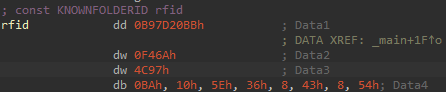
\includegraphics[width=0.7\textwidth]{resources/images/guid_in_assembly.png}
  \caption{A GUID in a binary disassembled by IDA Pro.}
  \label{fig:guid in assembly}
\end{figure}

To detect calls to \texttt{SHGetKnownFolderPath} that resolve the path used in \autoref{DP0}, we need to write a rule that constrains the specific bytes of the GUID in the first argument, like in \autoref{listing:call signature SHGetKnownFolderPath}.

\begin{lstlisting}[label={listing:call signature SHGetKnownFolderPath}, caption={A Call Signature that matches a call to \texttt{SHGetKnownFolderPath}.}, captionpos=b]
---

signature:
    technique: "DP0"
    description: >
      This Call Signature can be used to
      search for calls to SHGetKnownFolderPath.
    rules:
        - element: "function name"
          equals: "SHGetKnownFolderPath"

        - element: "number of arguments"
          equals: 4

        - element: "argument"
          argument_index: 0
          equals: "BB 20 7D B9 6A F4 97 4C BA 10 5E 36 08 43 08 54"
          type: "bytes"
\end{lstlisting}

\subsubsection{Deprecated API Functions}

Before Windows Vista, there were multiple (now deprecated, but still available) functions available to resolve the paths of directories.

All these functions take a constant that represents the startup directory as an argument. This constant is called \texttt{CSIDL\_STARTUP}\footnote{\tiny \url{https://docs.microsoft.com/en-us/windows/win32/shell/csidl}} and its value is 7.

\pagebreak

We write Call Signatures for all of these functions:
\begin{itemize}
    \item \texttt{SHGetFolderPath}\footnote{\tiny \url{https://docs.microsoft.com/en-us/windows/win32/api/shlobj_core/nf-shlobj_core-shgetfolderpathw}}
\begin{lstlisting}[caption={A Call Signature that matches a call to \texttt{SHGetFolderPath}.}, captionpos=b]
---

signature:
    technique: "DP0"
    description: >
      This Call Signature can be used to
      search for calls to SHGetFolderPath.
    rules:
        - element: "function name"
          contains: "SHGetFolderPath"

        - element: "number of arguments"
          equals: 5

        - element: "argument"
          argument_index: 1
          equals: 0x07
\end{lstlisting}


    \item \texttt{SHGetFolderLocation}\footnote{\tiny \url{https://docs.microsoft.com/en-us/windows/win32/api/shlobj_core/nf-shlobj_core-shgetfolderlocation}}
\begin{lstlisting}[caption={A Call Signature that matches a call to \texttt{SHGetFolderLocation}.}, captionpos=b]
---

signature:
    technique: "DP0"
    description: >
      This Call Signature can be used to
      search for calls to SHGetFolderLocation.
    rules:
        - element: "function name"
          contains: "SHGetFolderLocation"

        - element: "number of arguments"
          equals: 5

        - element: "argument"
          argument_index: 1
          equals: 0x07
\end{lstlisting}

\pagebreak

    \item \texttt{SHGetSpecialFolderPath}\footnote{\tiny \url{https://docs.microsoft.com/en-us/windows/win32/api/shlobj_core/nf-shlobj_core-shgetspecialfolderpathw}}:
\begin{lstlisting}[caption={A Call Signature that matches a call to \texttt{SHGetSpecialFolderPath}.}, captionpos=b]
---

signature:
    technique: "DP0"
    description: >
      This Call Signature can be used to
      search for calls to SHGetSpecialFolderPath.
    rules:
        - element: "function name"
          contains: "SHGetSpecialFolderPath"

        - element: "number of arguments"
          equals: 4

        - element: "argument"
          argument_index: 2
          equals: 0x07
\end{lstlisting}

    \item \texttt{SHGetSpecialFolderLocation}\footnote{\tiny \url{https://docs.microsoft.com/en-us/windows/win32/api/shlobj_core/nf-shlobj_core-shgetspecialfolderlocation}}:
\begin{lstlisting}[caption={A Call Signature that matches a call to \texttt{SHGetSpecialFolderLocation}.}, captionpos=b]
---

signature:
    technique: "DP0"
    description: >
      This Call Signature can be used to
      search for calls to SHGetSpecialFolderLocation.
    rules:
        - element: "function name"
          contains: "SHGetSpecialFolderLocation"

        - element: "number of arguments"
          equals: 3

        - element: "argument"
          argument_index: 1
          equals: 0x07
\end{lstlisting}
\end{itemize}

\section{Service-based Persistence Techniques}\label{section:call signatures sp}
In this section, we will discuss Call Signatures for \autoref{SP0}. As we discussed in \autoref{section:scheduled tasks services in windows}, there are multiple ways for an application to create a new service:

\begin{itemize}
    \item Calling the \texttt{CreateService} API function.
    \item Using the \texttt{sc.exe} command-line application.
    \item Writing directly to the Windows Registry.
\end{itemize}

\subsection{Creating Services Using the Windows API}
To create a service that is automatically started using the Windows API, an application needs to call the \texttt{CreateService} function.

The fifth argument of \texttt{CreateService} is a constant that signifies how the new service should be started. As malware wants the service to be started automatically, it uses the \texttt{SERVICE\_AUTO\_START}\footnote{\tiny \url{https://docs.microsoft.com/en-us/windows/win32/api/winsvc/nf-winsvc-createservicew}} constant. This constant has the value 2.

\autoref{listing:call signature CreateService} is a Call Signature that describes calls to \texttt{CreateService} with \texttt{SERVICE\_AUTO\_START} as the fifth argument.

\begin{lstlisting}[label={listing:call signature CreateService}, caption={A Call Signature that matches a call to \texttt{CreateService}.}, captionpos=b]
---

signature:
    technique: "SP0"
    description: >
      This Call Signature can be used to
      search for calls to CreateService.
    rules:
        - element: "function name"
          contains: "CreateService"

        - element: "number of arguments"
          equals: 13

        - element: "argument"
          argument_index: 5
          equals: 0x00000002
\end{lstlisting}

\subsection{Creating Services Using Sc.exe}\label{section:call signature sc.exe}
To create a service using the command line, malware needs to run the Sc.exe command. For example, the command in \autoref{listing:sc.exe command example}

\begin{lstlisting}[label={listing:sc.exe command example}, caption={An example usage of \texttt{sc.exe}.}, captionpos=b]
sc create ExampleService binpath="C:\temp\example.exe" start="auto" obj="LocalSystem"
\end{lstlisting}

To find such commands in a binary, we need a Call Signature that has rules for the two strings that will always be a part of these commands: ``sc'' and ``create''. The Call Signature in \autoref{listing:call signature sc.exe} has these rules.

\begin{lstlisting}[label={listing:call signature sc.exe}, caption={A Call Signature that matches creating a service using the \texttt{sc.exe} application.}, captionpos=b]
---

signature:
    technique: "SP0"
    description: >
      This Call Signature can be used to
      search for usage of sc.exe commands.
    rules:
      - element: "any argument"
        contains: "sc"

      - element: "any argument"
        contains: "create"
\end{lstlisting}

\subsection{Creating Services Using the Registry}
The configuration of services is stored in the Registry in the key \path{HKLM\SYSTEM\CurrentControlSet\Services}. It is possible to write to a subkey of this key directly, to create a new service.

To be able to detect this, we will use the same Call Signatures as in \autoref{section:call signatures rp}, but we will use \path{HKLM\SYSTEM\CurrentControlSet\Services} (instead of \path{HKCU\SOFTWARE\Microsoft\Windows\CurrentVersion\Run}).

\section{Scheduled Tasks-based Persistence Techniques}\label{section:call signatures tp}
In this section, we will discuss Call Signatures for \autoref{TP0}. As we discussed in \autoref{section:scheduled tasks services in windows}, there are multiple ways for an application to create a scheduled task:

\begin{itemize}
    \item Directly calling Windows API functions.
    \item Using the \texttt{schtasks.exe} command-line application.
    \item Using the \texttt{at.exe} command-line application.
\end{itemize}

\subsection{Creating Services Using the Windows API}
To create a scheduled task using the Windows API directly, an application needs to interact with the Task Scheduler service. The Windows API provides two ways to achieve this. Both use the \texttt{CoCreateInstance} to create a handler for the Task Scheduler service.

The first method calls \texttt{CoCreateInstance} with the following constants as its arguments. These constants are GUIDs (discussed in \autoref{section:call signatures dp}) The values of the first and fourth argument are:
\begin{itemize}
  \item \texttt{CLSID\_CTaskScheduler}: \texttt{148BD52A-A2AB-11CE-B11F-00AA00530503}
  \item \texttt{IID\_ITaskScheduler}: \texttt{148BD527-A2AB-11CE-B11F-00AA00530503}
\end{itemize}

The second, newer method is similar to the first, but uses different constants:
\begin{itemize}
  \item \texttt{CLSID\_TaskScheduler}: \texttt{0F87369F-A4E5-4CFC-BD3E-73E6154572DD}
  \item \texttt{IID\_ITaskService}: \texttt{2FABA4C7-4DA9-4013-9697-20CC3FD40F85}
\end{itemize}

\autoref{listing:call signature CoCreateInstance} shows a Call Signature that has rules to constrain these constants.

\begin{lstlisting}[label={listing:call signature CoCreateInstance}, caption={A Call Signature that matches a call to \texttt{CoCreateInstance}.}, captionpos=b]
---

signature:
    technique: "TP0"
    description: >
      This Call Signature can be used to
      search for calls to CoCreateInstance.
    rules:
        - element: "function name"
          equals: "CoCreateInstance"

        - element: "number of arguments"
          equals: 5

        - element: "argument"
          argument_index: 0
          in:
            - "2A D5 8B 14 AB A2 CE 11 B1 1F 00 AA 00 53 05 03"
            - "9F 36 87 0F E5 A4 FC 4C BD 3E 73 E6 15 45 72 DD"
          type: "bytes"

        - element: "argument"
          argument_index: 3
          in:
            - "27 D5 8B 14 AB A2 CE 11 B1 1F 00 AA 00 53 05 03"
            - "C7 A4 AB 2F A9 4D 13 40 96 97 20 CC 3F D4 0F 85"
          type: "bytes"
\end{lstlisting}

\subsection{Creating Services Using Schtasks.exe}
It is also possible to create a scheduled task using the command line, with the schtasks.exe application. For example, the command in \autoref{listing:schtasks.exe command example}.

\begin{lstlisting}[label={listing:schtasks.exe command example}, caption={An example \texttt{schtasks.exe} command that runs a fictitious executable when a user is idle for 30 minutes.}, captionpos=b]
schtasks /create /tn WindowsUpdate /tr "c:\windows\real_update.exe /sc onidle /i 30
\end{lstlisting}

Similar to sc.exe in \autoref{section:call signature sc.exe}, we need rules that capture the strings that will always be part of the command: ``schtasks'' and ``/create''. Like the Call Signature in \autoref{listing:call signature schtasks.exe}.

\begin{lstlisting}[label={listing:call signature schtasks.exe}, caption={A Call Signature that matches creating a scheduled task using the \texttt{schtasks.exe} application.}, captionpos=b]
---

signature:
    technique: "TP0"
    description: >
      This Call Signature can be used to
      search for usage of schtasks.exe commands.
    rules:
        - element: "any argument"
          contains: "schtasks"

        - element: "any argument"
          contains: "/create"
\end{lstlisting}

\subsection{Creating Services Using At.exe}
The Call Signature for at.exe is similar to the one for schtasks.exe because the applications themselves are similar. \autoref{listing:at.exe command example} shows an example of an at.exe command.

\begin{lstlisting}[label={listing:at.exe command example}, caption={An example \texttt{at.exe} command that runs a fictitious executable every Monday at 9:00.}, captionpos=b]
at 09:00 /interactive /every:m C:\Windows\System32\WindowsUpdate\reverseshell.exe
\end{lstlisting}

To be able to find function calls that perform some operation on such commands, we need to find all occurrences of ``at'' and ``/every''.

\begin{minipage}{0.9\textwidth}
\begin{lstlisting}[label={listing:call signature at.exe}, caption={A Call Signature that matches creating a scheduled task using the \texttt{at.exe} application.}, captionpos=b]
---

signature:
    technique: "TP0"
    description: >
      This Call Signature can be used to
      search for usage of at.exe commands.
    rules:
        - element: "any argument"
          contains: "at"

        - element: "any argument"
          contains: "/every:"
\end{lstlisting}
\end{minipage}

\section{A Reflection on Writing Call Signatures}\label{section:reflection on writing call signatures}
After writing the Call Signatures for this chapter, we wanted to share some thoughts on the process of writing Call Signatures.

Generally speaking, Call Signatures are quite expressive. We were able to express every constraint on function call elements we wanted, with a relatively small number of operators and types.

Especially only supporting three types (strings, numbers, and bytes) seemed to be enough to cover all situations we want. This is likely because many API functions use constants as arguments. Besides this, interesting arguments are often strings (e.g. Registry paths and commands for the command line).

\medskip

In an earlier iteration of Call Signatures, we included the return type as a function call element. However, we noticed that we never used a constraint on the return type when writing Call Signatures. The return type was not needed, because the only times we know the return type is for Windows API functions, and we were already able to search for these using the function name. Writing rules that constraint the function name and arguments was enough for us.

\medskip

In \autoref{section:call signatures dp}, we wrote Call Signatures for multiple similar API functions that are used to resolve paths. This resulted in multiple Call Signatures with only slight differences. It would be a good improvement to be able to combine these into one Call Signature.

\medskip

Unfortunately, string parameters are not always passed directly into calls. Sometimes, they are first manipulated in some way. For example, they are turned into \texttt{CString} objects\footnote{\tiny \url{https://docs.microsoft.com/en-us/cpp/atl-mfc-shared/using-cstring}} or formatted using \texttt{cprintf}\footnote{\tiny \url{https://www.cplusplus.com/references/cstdio/printf/}}. To capture such situations, we wrote Call Signatures to search for function calls to unspecified functions with a string as one of their arguments. For example, the Call Signatures in \autoref{listing:call signature run key reg.exe} and \autoref{listing:call signature schtasks.exe}. This allows us to detect many calls to functions that perform some action on a string of interest. This does however increase the chance of false positives.

